\scanpage{113}

\uline{Théorème de Bertini et variantes}.

Dans la suite $k$ désigne un corps, $P^r=P^r_k$.

\margin{\figure{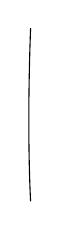
\begin{tikzpicture}\draw (0,0) .. controls (-.03,-.8) and (-.03,-1.6) .. (0,-2.2);\end{tikzpicture}}}
\uline{Théorème de Bertini} 1: Soit $f:X\handwritten{\rightarrow}P^r_k$ un morphisme, où $X$ est un schéma algébrique géométriquement irréductible, et soit $n=\dim\overset{\handwritten{\rule{1.9em}{.4pt}}}{f(X)}$. Soit $L_t$ le\deleted{\unsure{s|un}} sous-espace linéaire de codimension $s$ \uline{générique} de $P^r$, où $s$ est un entier fixé $\handwritten{\leq}n-1$. Alors $\inserted{Y_t=}f_t^{-1}(L_t)\handwritten{\subset}X_t=X\otimes_k k(t)$ est géométriquement irréductible.
% The bar above f(X) is handwritten.

% This marginal note is slanted upward on the original.
\margin{\handwritten{\unsure{vrai} dans\\\unsure{E|S}GA \unsure{V|IV}}\figure{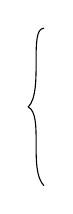
\begin{tikzpicture}\draw (.2,0) .. controls (0,0) and (.2,-.8) .. (0,-1) .. controls (.2,-1.1) and (0,-1.8) .. (.2,-2);\end{tikzpicture}}}
\margin{\figure{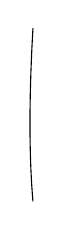
\begin{tikzpicture}\draw (0,0) .. controls (-.04,-.7) and (-.06,-1.5) .. (0,-2.2);\end{tikzpicture}}}
\inserted{Enoncé local 2: Soit $f:X\handwritten{\rightarrow}P^r$ un morphisme, avec $X$ un schéma algébrique.} \deleted{\uline{Complément:} Supposons} Soit $Z\handwritten{\rightarrow}X$ \deleted{\illegible{2}} l'ensemble des points de $X$ en lesquels \inserted{\handwritten{soit}} $f$ est \deleted{\handwritten{soit}} ramifié \deleted{ou en lesquels} \inserted{\handwritten{soit}} $X$ n'est pas géométriquement unibranche (resp.\ \inserted{\handwritten{pas}} normal, resp.\ \inserted{\handwritten{pas}} lisse \ldots), \deleted{alors} et supposons que $\overset{\handwritten{\rule{1.9em}{.4pt}}}{f(Z)}$ soit de dimension $\handwritten{<}s$. Alors $\inserted{Y_t=}f_t^{-1}(L_t)$ est géométriquement unibranche (resp.\ normal, resp.\ lisse \ldots), où $L_t$ est comme ci-dessus.
% The bar above f(Z) is handwritten. The underline under the old Complément:
% ends before the end of the inserted words Enoncé local; no separate
% underline of that inserted heading is securely visible.

De ces deux énoncés on déduit\handwritten{/}formellement;

\margin{\figure{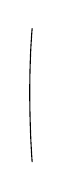
\begin{tikzpicture}\draw (0,0) .. controls (-.05,-.6) and (-.03,-1.3) .. (0,-1.7);\end{tikzpicture}}}
% The cancelled é shares its cell with the C of Corollaire.
\deleted{Thé}\uline{Corollaire} 3: Soit $f:X\handwritten{\longrightarrow}P^r$ satisfaisant les conditions de 1\handwritten{,} et 2 non respé.\ \inserted{Supposons $k$ alg.\ clos.} Alors le\deleted{inclusion} morphisme canonique
\[
\handwritten{\pi}_1(Y_{\bar{t}})\handwritten{\rightarrow}\handwritten{\pi}_1(X)
\]
est surjectif.

% Unlike-letter contours coexist in the marked interior cells, and the
% numeral contains 3/4 contours without an established correction order.
\uline{Re\unsure{ma}\unsure{r|q}que} \unsure{3|4}. Utilisant les théorèmes de changement de base pour le $\handwritten{\pi}_1$, on conclut \deleted{que} (posant $X_{\bar{t}}=X\otimes_k k(\bar{t})$) que l'homomorphisme $\deleted{\unsure{\pi}_1(}$
\[
\handwritten{\pi}_1(Y_{\bar{t}})\handwritten{\rightarrow}\handwritten{\pi}_1(X_{\bar{t}})\tag*{\makebox[0pt][r]{\makebox[\linewidth][l]{(*)}}}
\]
est surjectif si $X_{\deleted{\unsure{t|\bar{t}}}}$ est propre, et que l'homomorphisme
\[
\handwritten{\pi}_1^{!}(\unsure{X|Y}_{\bar{t}})\handwritten{\rightarrow}\handwritten{\pi}_1^{!}(X_{\bar{t}})\tag*{\makebox[0pt][r]{\makebox[\linewidth][l]{\handwritten{(**)}}}}
\]
% Both written display labels are at the left margin.
% The first source letter in (**) is an X/Y composite; chronology is not established.
est surjectif, où le ! désigne le plus grand quotient profini premier à l'è\unsure{d|x}posant car.\ de $k$. On n'affirme pas, cependant, que (*) soit toujours surjectif (sans hypothèse de propreté sur $X$).
% The d/x cell contains both contours; no deletion order is asserted.

On déduit, de 1, par une application facile du théorème de connexité:

% V below inherits the upper note's V/IV ambiguity under the recurrence rule.
\margin{\handwritten{vu. dans\\EGA V}\figure{\begin{tikzpicture}\draw (0,0)--(.03,-.5);\end{tikzpicture}}}
\uline{Corollaire} 4 (de 1): Sous les conditions de 1) pour $f:X\handwritten{\longrightarrow}P^r$, si $X$
% archive sheet number: 112
